%%__________________________________________________________________||

%%__________________________________________________________________||
\RCS$Revision: 310955 $
\RCS$HeadURL: svn+ssh://svn.cern.ch/reps/tdr2/notes/SUS-15-005/trunk/SUS-15-005.tex $
\RCS$Id: SUS-15-005.tex 310955 2015-11-17 23:57:25Z sakuma $

%%__________________________________________________________________||
\cmsNoteHeader{SUS-15-005}

%%__________________________________________________________________||
\title{Search for new physics in final states with jets and missing
transverse momentum in $\sqrt{s}$ = 13~TeV pp collisions with the
$\alpha_{\text{T}}$ variable}

%%__________________________________________________________________||
\address[cern]{CERN}
\author[cern]{The CMS Collaboration}

%%__________________________________________________________________||
\date{\today}

%%__________________________________________________________________||
\abstract{An inclusive search for supersymmetric processes that produce
final states with jets and missing transverse momentum is performed in pp
collisions at a centre-of-mass energy of 13 TeV. A dimensionless
kinematic variable, $\alpha_{\text{T}}$, is used to discriminate between
events with genuine and misreconstructed missing transverse momentum. A
data sample corresponding to an integrated luminosity of
2.1~$\text{fb}^{-1}$, recorded by the CMS experiment at the LHC, is
analysed. The observed signal candidate event counts are found to be in
agreement with the expected contributions from standard model processes
and the result is interpreted in the parameter space of simplified
models.}

% 1. **DO NOT use \include or \input** to include the abstract: our
%    abstract extractor will not search through other files than this
%    one.
% 2. **DO NOT use %** to comment out sections of the abstract: the
%    extractor will still grab those lines (and they won't be
%    comments any longer!).
% 3. For PASs: **DO NOT use tex macros** in the abstract: CDS MathJax
%    processor used on the abstract doesn't understand them _and_ will
%    only look within $$. The abstracts for papers are hand formatted
%    so macros are okay.


%%__________________________________________________________________||
%\newcommand{\eslash}{{\hbox{$E$\kern-0.6em\lower-.05ex\hbox{/}\kern0.10em}}}
\newcommand{\met}{\mbox{$\eslash_\text{T}$}\xspace}
\newcommand{\cls}{\mbox{CL$_s$}\xspace}
\newcommand{\wtaunu}{\ensuremath{\PW \rightarrow \Pgt\cPgn}}
\newcommand{\Et}{\ensuremath{{E_{\text T}}}\xspace}
\newcommand{\Hslash}{{\hbox{$H$\kern-0.8em\lower-.05ex\hbox{/}\kern0.10em}}}

\newcommand{\scalht}{\mbox{$H_\text{T}$}\xspace}
\newcommand{\mht}{\mbox{$\Hslash_\text{T}$}\xspace}
\newcommand{\HTmiss}{\mbox{$H_\text{T}^\text{miss}$}\xspace}
\newcommand{\dht}{\ensuremath{\Delta\scalht}\xspace}
\newcommand{\alphat}{\ensuremath{\alpha_{\text T}}\xspace}
\newcommand{\njet}{\ensuremath{N_{\text{jet}}}\xspace}
\newcommand{\njetlow}{\ensuremath{2 \leq \njet \leq 3}\xspace}
\newcommand{\njethigh}{\ensuremath{\njet \geq 4}\xspace}
\newcommand{\nb}{\ensuremath{N_{\text{b}}}\xspace}
\newcommand{\mj}{\ensuremath{\mu\! +\! \text{jets}}\xspace}
\newcommand{\mmj}{\ensuremath{\mu\mu\! +\! \text{jets}}\xspace}
\newcommand{\gj}{\ensuremath{\gamma\! +\! \text{jets}}\xspace}
\newcommand{\wjets}{\ensuremath{\PW\! +\! \text{jets}}\xspace}
\newcommand{\zjets}{\ensuremath{\cPZ\! +\! \text{jets}}\xspace}
\newcommand{\znunujets}{\ensuremath{\cPZ\! \rightarrow\! \cPgn\cPagn\! +\! \text{jets}}\xspace}
\newcommand{\znunu}{\ensuremath{\cPZ\! \rightarrow\! \cPgn\cPagn}\xspace}
\newcommand{\zmumu}{\ensuremath{\cPZ\! \rightarrow\! \mu\mu}\xspace}
\newcommand{\zmumujets}{\ensuremath{\cPZ\! \rightarrow\! \mu\mu\! +\! \text{jets}}\xspace}
\newcommand\T{\rule{0pt}{2.6ex}}
\newcommand\B{\rule[-1.2ex]{0pt}{0pt}}
\def\mhtmet{\mbox{$\HTmiss / \ETmiss$}\xspace}
\newcommand{\Pt}{\ensuremath{{p_{\text T}}}\xspace}
\newcommand{\dphi}{\ensuremath{\Delta\phi^{*}_\text{min}}\xspace}
\newcommand{\dm}{\ensuremath{\Delta m}\xspace}
\newcommand{\alphatmin}{\ensuremath{\alphat^\text{min}}\xspace}

%\newcommand\rs{\raisebox{1.0ex}[-1.0ex]}

% PROCESSES

\newcommand{\ra}{\ensuremath{\rightarrow}}
\newcommand{\jets}{\ensuremath{\text{jets}}}

\newcommand{\lj}{\ensuremath{\ell\! +\! \jets}\xspace}
\newcommand{\mj}{\ensuremath{\mu\! +\! \jets}\xspace}
\newcommand{\ej}{\ensuremath{e\! +\! \jets}\xspace}

\newcommand{\llj}{\ensuremath{\ell\ell\! +\! \jets}\xspace}
\newcommand{\mmj}{\ensuremath{\mu\mu\! +\! \jets}\xspace}
\newcommand{\eej}{\ensuremath{ee\! +\! \jets}\xspace}
\newcommand{\mmjpm}{\ensuremath{\mu^\pm\mu^\mp\! +\! \jets}\xspace}

\newcommand{\gj}{\ensuremath{\gamma\! +\! \jets}\xspace}

\newcommand{\wj}{\ensuremath{\PW\! +\! \jets}\xspace}
\newcommand{\wlj}{\ensuremath{\PW\! (\ra\! \ell\nu)\! +\! \textrm{jets}}\xspace}
\newcommand{\wmj}{\ensuremath{\PW\! (\ra\! \mu\nu)\! +\! \textrm{jets}}\xspace}
\newcommand{\wej}{\ensuremath{\PW\! (\ra\! e\nu)\! +\! \textrm{jets}}\xspace}

\newcommand{\wlnu}{\ensuremath{\PW\! \ra\! \ell\nu}\xspace}
\newcommand{\wmunu}{\ensuremath{\PW\! \ra\! \mu\nu}\xspace}
\newcommand{\wenu}{\ensuremath{\PW\! \ra\! e\nu}\xspace}
\newcommand{\wtaunu}{\ensuremath{\PW \rightarrow \Pgt\cPgn}\xspace}

\newcommand{\zj}{\ensuremath{\cPZ\! +\! \jets}\xspace}
\newcommand{\zllj}{\ensuremath{\cPZ\! (\ra\! \ell\ell)\! + \! \jets}\xspace}
\newcommand{\zmumuj}{\ensuremath{\cPZ\! (\ra\! \mu\mu)\! +\! \jets}\xspace}
\newcommand{\zeej}{\ensuremath{\cPZ\! (\ra\! ee)\! +\! \jets}\xspace}
\newcommand{\znunuj}{\ensuremath{\cPZ\! (\ra\! \cPgn\cPagn)\! +\! \jets}\xspace}

\newcommand{\zll}{\ensuremath{\cPZ\! \ra\! \ell\ell}\xspace}
\newcommand{\zmumu}{\ensuremath{\cPZ\! \ra\! \mu\mu}\xspace}
\newcommand{\zee}{\ensuremath{\cPZ\! \ra\! ee}\xspace}
\newcommand{\znunu}{\ensuremath{\cPZ\! \ra\! \cPgn\cPagn}\xspace}

\newcommand{\ttj}{\ensuremath{\ttbar\! +\! \jets}\xspace}
\newcommand{\ttw}{\ensuremath{\ttbar\PW}\xspace}
\newcommand{\ttz}{\ensuremath{\ttbar\cPZ}\xspace}

% SIGNAL 

\newcommand{\Ttwocc}{\ensuremath{\text{pp}\,\ra\,\sTop\sTop^{*}\,\ra\,\text{c}\chiz\,\bar{\text{c}}\chiz}}
\newcommand{\Ttwodegen}{\ensuremath{\text{pp}\,\ra\,\sTop\sTop^{*}\,\ra\,\text{b}ff'\chiz \,\text{b}ff'\chiz}}
\newcommand{\Ttwobw}{\ensuremath{\text{pp}\,\ra\,\sTop\sTop^{*}\,\ra\,\text{b}W\chiz \,\bar{\text{b}}W\chiz}}
\newcommand{\Ttwott}{\ensuremath{\text{pp}\,\ra\,\sTop\sTop^{*}\,\ra\,\text{t}\chiz\,\bar{\text{t}}\chiz}}
\newcommand{\Ttwobb}{\ensuremath{\text{pp}\,\ra\,\sBot\sBot^{*}\,\ra\,\text{b}\chiz\,\bar{\text{b}}\chiz}}
\newcommand{\Ttwoqq}{\ensuremath{\text{pp}\,\ra\,\sQua\sQua^{*}\,\ra\,\text{q}\chiz\,\bar{\text{q}}\chiz}}
\newcommand{\Tonebbbb}{\ensuremath{\text{pp}\,\ra\,\sGlunew\sGlunew^{*}\,\ra\,\bar{\text{b}}\text{b}\chiz\,\bar{\text{b}}\text{b}\chiz}}
\newcommand{\Toneqqqq}{\ensuremath{\text{pp}\,\ra\,\sGlunew\sGlunew^{*}\,\ra\,\bar{\text{q}}\text{q}\chiz\,\bar{\text{q}}\text{q}\chiz}}
\newcommand{\Tonetttt}{\ensuremath{\text{pp}\,\ra\,\sGlunew\sGlunew^{*}\,\ra\,\bar{\text{t}}\text{t}\chiz\,\bar{\text{t}}\text{t}\chiz}}

%\newcommand{\dphi}{\ensuremath{\Delta \phi}}
\newcommand{\dphi}{\ensuremath{\Delta\phi^{*}_{\rm min}}\xspace}
\newcommand{\dphijj}{\ensuremath{\Delta \phi_{ j1,j2}}}
\newcommand{\Pt}{\ensuremath{{p_{\text T}}}\xspace}
\newcommand{\pts}{\ensuremath{p_{\text T}{\text s}}\xspace}
\newcommand{\Et}{\ensuremath{{E_{\text T}}}\xspace}
\newcommand{\ptjf}{\ensuremath{p_{\rm T}^{ {\rm j}_1} }}
\newcommand{\ptjs}{\ensuremath{p_{\rm T}^{ {\rm j}_2} }}
\newcommand{\ptjt}{\ensuremath{p_{\rm T}^{ {\rm j}_3} }}
\newcommand{\etajf}{\ensuremath{\eta^{ {\rm j}_1} }}
\newcommand{\etajs}{\ensuremath{\eta^{ {\rm j}_2} }}
\newcommand{\etajt}{\ensuremath{\eta^{ {\rm j}_3} }}
\newcommand{\al}{\ensuremath{\alpha}}
\newcommand{\alt}{\ensuremath{\alpha_{\text{T}}}\xspace}
\newcommand{\etaabs}{\ensuremath{|\eta|}}
%\newcommand{\gev}{\ensuremath{\mathrm{\,Ge\kern -0.1em V}}}
\newcommand{\pb}{\ensuremath{pb^{-1}}}
\newcommand{\mjj}{\ensuremath{M_{\text{inv}}^{j1,j2}}}
\newcommand{\chiznew}{\ensuremath{\chi^{0}}\xspace}
\newcommand{\chipnew}{\ensuremath{\chi^{+}}\xspace}
\newcommand{\sQuanew}{\ensuremath{\tilde{\rm q}}\xspace}
\newcommand{\sGlunew}{\ensuremath{\tilde{\rm g}}\xspace}
\newcommand{\ttNew}{\ensuremath{\rm{t}\bar{\rm{t}}}\xspace}
\newcommand{\tev}{\TeV}
%<TW date="30/10/2010">
%\newcommand{\Et}{E_{T}}
\newcommand{\combIso}{Iso_{\textrm{comb.}}}
\renewcommand{\arraystretch}{1.2}
\newcommand{\bigNum}[2]{#1 \, \times \, 10 \, ^{#2}}
%</TW>

\newcommand{\raT}{\ensuremath{R_{\alt}}}
\newcommand{\RaT}{\ensuremath{R_{\alt}}\xspace}

\newcommand\T{\rule{0pt}{2.6ex}}
\newcommand\B{\rule[-1.2ex]{0pt}{0pt}}

\def\eslash{{\hbox{$E$\kern-0.6em\lower-.05ex\hbox{/}\kern0.10em}}}
\def\vecmet{\mbox{$\vec{\eslash}_T$}} %missing ET vector
\def\vecet{\mbox{$\vec{E}_\text{T}$}} % ET vector
\def\MET{\mbox{$\eslash_\text{T}$}\xspace}
%\def\met{\mbox{$\eslash_\text{T}$}\xspace}
\def\met{\mbox{$E_\text{T}^{\rm miss}$}\xspace}
\def\pfmet{\mbox{$\eslash_\text{T}^{\rm PF}$}\xspace}
\def\mex{\mbox{$\eslash_\text{x}$}} %missing Ex
\def\mey{\mbox{$\eslash_\text{y}$}} %missing Ey
\def\mepar{\mbox{$\eslash_\parallel$}}
\def\meperp{\mbox{$\eslash_\perp$}}
\def\Zmm{Z \rightarrow \mu\mu}
\def\metvec{\mbox{$\vec{\met}$}\xspace}
\def\metvecrec{\mbox{$\vec{\met}^{\rm rec}$}\xspace}
\def\metvecgen{\mbox{$\vec{\met}^{\rm gen}$}\xspace}
\def\metgen{\mbox{$\met^{\rm gen}$}\xspace}
\def\metparl{\mbox{$\mepar^{\rm rec}$}\xspace}
\def\metperp{\mbox{$\meperp^{\rm rec}$}\xspace}
\def\deltamet{\mbox{$\Delta\met$}\xspace}
\def\pthat{\mbox{$\hat{p}_T$}\xspace}
\def\hslash{{\hbox{$H$\kern-0.8em\lower-.05ex\hbox{/}\kern0.10em}}}
%\def\MHT{\mbox{$\hslash_\text{T}$}\xspace}
\def\mht{\mbox{$\hslash_\text{T}$}\xspace}
%\def\mht{\mbox{$H_{\rm T}^{\rm miss}$}\xspace}
\newcommand{\HTmiss}{\ensuremath{H_{\text{T}}^{\text{miss}}}\xspace}
\newcommand{\HTmissvec}{\ensuremath{\vec{H_{\text{T}}}^{\text{miss}}}\xspace}
\def\mhtvec{\mbox{$\vec{H}_{\rm T}^{\rm miss}$}\xspace}
%\def\mhtmet{\mbox{$\hslash_\text{T} / \eslash_\text{T}$}\xspace}
%\def\mhtmet{\mbox{$\mht / \met$}\xspace}
\newcommand{\mhtmet}{\ensuremath{H_{\mathrm{T}}^{\text{miss}} / E_{\mathrm{T}}^{\text{miss}}}\xspace}
\def\mhtmetmiss{\mbox{$\H_\text{T}^{\rm miss} / \E_\text{T}^{\rm miss}$}\xspace}
%\def\rmhtmet{\mbox{$R_{\hslash_\text{T} / \eslash_\text{T}}$}\xspace}
\def\rmhtmet{\mbox{$R_{\mht / \met}$}\xspace}
\def\sumet{\mbox{$\sum \rm{E}_\text{T}$}\xspace}
\def\etmiss{\mbox{$\eslash_\text{T}$}\xspace}
\def\htmiss{\mbox{$\hslash_\text{T}$}\xspace}
\def\mtt{\mbox{$\rm{M}_\text{T2}$}\xspace}
\def\rmec{\mbox{$R_{\mht/\met}$}\xspace}
\def\bdphi{\mbox{$\Delta\phi^{*}_{\rm min}$}\xspace}
\def\bdphimod{\mbox{$\Delta\phi^{*_{\, 25}}_{\rm min}$}\xspace}
\def\bigeslash{{\hbox{$E$\kern-0.38em\lower-.05ex\hbox{/}\kern0.10em}}}
\def\bigmet{\mbox{$\bigeslash_T$}}
\def\bighslash{{\hbox{$H$\kern-0.6em\lower-.05ex\hbox{/}\kern0.10em}}}
\def\bigmht{\mbox{$\bighslash_T$}}
\def\incl{\includegraphics[width=0.49\linewidth]}
\def\inclrot{\includegraphics[angle=90,width=0.47\linewidth]}
\def\INCL{\includegraphics[angle=90,width=0.45\linewidth]}
\def\Incl{\includegraphics[angle=90,width=0.60\linewidth]}
\def\cls{\mbox{CL$_s$}\xspace}

\newcommand{\zero}{\ensuremath{\phantom{0}}}

\newcommand{\scalht}{\ensuremath{H_{\mathrm{T}}}\xspace}
\newcommand{\dm}{\ensuremath{\Delta m}\xspace}


%%__________________________________________________________________||
\newlength\cmsFigWidth
\ifthenelse{\boolean{cms@external}}{\setlength\cmsFigWidth{0.85\columnwidth}}{\setlength\cmsFigWidth{0.4\textwidth}}
\ifthenelse{\boolean{cms@external}}{\providecommand{\cmsLeft}{top\xspace}}{\providecommand{\cmsLeft}{left\xspace}}
\ifthenelse{\boolean{cms@external}}{\providecommand{\cmsRight}{bottom\xspace}}{\providecommand{\cmsRight}{right\xspace}}

\newcommand{\eslash}{{\hbox{$E$\kern-0.6em\lower-.05ex\hbox{/}\kern0.10em}}}
\newcommand{\met}{\mbox{$\eslash_\text{T}$}\xspace}
\newcommand{\cls}{\mbox{CL$_s$}\xspace}
\newcommand{\wtaunu}{\ensuremath{\PW \rightarrow \Pgt\cPgn}}
\newcommand{\Et}{\ensuremath{{E_{\text T}}}\xspace}
\newcommand{\Hslash}{{\hbox{$H$\kern-0.8em\lower-.05ex\hbox{/}\kern0.10em}}}

\newcommand{\scalht}{\mbox{$H_\text{T}$}\xspace}
\newcommand{\mht}{\mbox{$\Hslash_\text{T}$}\xspace}
\newcommand{\dht}{\ensuremath{\Delta\scalht}\xspace}
\newcommand{\alphat}{\ensuremath{\alpha_{\text T}}\xspace}
\newcommand{\njet}{\ensuremath{n_{\text{jet}}}\xspace}
\newcommand{\njetlow}{\ensuremath{2 \leq \njet \leq 3}\xspace}
\newcommand{\njethigh}{\ensuremath{\njet \geq 4}\xspace}
\newcommand{\nb}{\ensuremath{n_{\text{b}}}\xspace}
\newcommand{\mj}{\ensuremath{\mu + \text{jets}}\xspace}
\newcommand{\mmj}{\ensuremath{\mu\mu + \text{jets}}\xspace}
\newcommand{\gj}{\ensuremath{\gamma + \text{jets}}\xspace}
\newcommand{\znunu}{\ensuremath{\cPZ \rightarrow \cPgn\cPagn}\xspace}
\newcommand{\zmumu}{\ensuremath{\cPZ \rightarrow \mu\mu}\xspace}
\newcommand\T{\rule{0pt}{2.6ex}}
\newcommand\B{\rule[-1.2ex]{0pt}{0pt}}
\def\mhtmet{\mbox{$\Hslash_\text{T} / \eslash_\text{T}$}\xspace}
\newcommand{\Pt}{\ensuremath{{p_{\text T}}}\xspace}
\newcommand{\dphi}{\ensuremath{\Delta\phi^{*}_{\rm min}}\xspace}
\newcommand{\dm}{\ensuremath{\Delta m}\xspace}

%%__________________________________________________________________||
\hypersetup{
pdfauthor={Mark Baber, Robert Bainbridge, Freya Blekman, Oliver
Buchmueller, Jim Brooke, Stefano Casasso, Matthew Citron, Adam Elwood,
Henning Flaecher, Aran Garcia-Bellido, Christian Laner, Kin Ho Lo,
Sarah Alam Malik, Bjoern Penning, Tai Sakuma, Dominic Smith, Alex
Tapper},
pdftitle={Search for new physics in final states with jets and missing
transverse momentum in sqrt(s) = 13 TeV pp collisions with the alphaT
variable},
pdfsubject={CMS},
pdfkeywords={CMS, jets, missing transverse momentum, supersymmetry,
dark matter, AlphaT}
}


%%__________________________________________________________________||
\maketitle

%%__________________________________________________________________||
% \tableofcontents

%%__________________________________________________________________||
\section{Introduction}
\label{sec:introduction}

The standard model (SM) of particle physics is widely considered to be
only an effective approximation of a more complete theory, such as
supersymmetry (SUSY)~\cite{ref:SUSY-1,ref:SUSY0,ref:SUSY1,ref:SUSY2,ref:SUSY3,ref:SUSY4,ref:hierarchy1,ref:hierarchy2},
that would supersede the SM at a higher energy scale. For R-parity conserving
SUSY~\cite{Farrar:1978xj}, supersymmetric particles (sparticles) such
as squarks and gluinos are produced in pairs and decay to the
lightest, stable supersymmetric particle (LSP), which is generally
assumed to be a weakly interacting and massive neutralino, the $\chiz_1$. 
A characteristic signature is a final state of multijets accompanied by
significant missing transverse momentum, $\ptvecmiss$.

This document presents an inclusive search for the pair production of
massive coloured sparticles in hadronic final states with two or more
energetic jets and \met, performed in pp collisions at a
centre-of-mass energy $\sqrt{s} = 13\TeV$. The analysed data sample
corresponds to an integrated luminosity of $2.1 \pm 0.3
\fbinv$~\cite{lumi} collected by the Compact Muon Solenoid (CMS)
experiment. Previous iterations of this search have been performed in
pp collisions at both $\sqrt{s} = 7$~\cite{RA1Paper, RA1Paper2011,
  RA1Paper2011FULL} and $8\TeV$~\cite{RA1Paper2012}.


The search is devised around the kinematic variable
\alphat~\cite{Randall:2008rw, RA1Paper} that provides powerful
discrimination against multijet production, a manifestation of quantum
chromodynamics (QCD), and adheres to an inclusive strategy with the
aim of providing sensitivity to the widest possible range of SUSY
models. The \alphat variable is constructed from jet-based quantities
to provide robust discriminating power between sources of genuine and
misreconstructed missing transverse momentum, making it suitable for early
searches. A further variable that exploits azimuthal angular
information, known as $\Delta\phi^{*}_{\rm min}$~\cite{RA1Paper}, is
also employed to suppress QCD multijet production, including potential
contributions from semileptonic heavy-flavour decays, to a negligible
level.

The search is based on an examination of the number of reconstructed
jets per event, the scalar (\scalht) and vector (\mht) sums of
transverse momenta of these jets, and the number of these jets
identified as originating from bottom quarks. The search exploits the
use of \mht templates derived from simulation, which are extensively
validated in data control regions. These discriminating variables
provide sensitivity to the different production mechanisms of massive
coloured sparticles at hadron colliders (\ie squark-squark,
squark-gluino, and gluino-gluino), a large range of mass splittings
between the parent sparticle and the LSP, and third-generation squark
signatures, respectively. Interpretations of the analysis are provided
in the parameter space of simplified models~\cite{Alwall:2008ag,
  Alwall:2008va, sms}. Limits are derived in the mass parameter space
of simplified models of pair-produced gluinos, decaying inclusively to
four quarks and additionally decaying to four top and bottom
quarks. Figure~\ref{fig:feyn} illustrates the simplified models
considered.

\begin{figure*}[thb]
\centering
\includegraphics[width=0.32\linewidth]{T1bbbb.pdf}
\includegraphics[width=0.32\linewidth]{T1tttt.pdf}
\includegraphics[width=0.32\linewidth]{T1qqqq.pdf}
\caption{
Feynman diagrams for the simplified models.
}
\label{fig:feyn}
\end{figure*}


%%__________________________________________________________________||

%%__________________________________________________________________||
\section{The CMS detector}
\label{sec:detector}

% https://twiki.cern.ch/twiki/bin/viewauth/CMS/Internal/PubDetector

The central feature of the CMS apparatus is a superconducting solenoid
of 6\unit{m} internal diameter, providing a magnetic field of
3.8\unit{T}. Within the superconducting solenoid volume are a silicon
pixel and strip tracker, a lead tungstate crystal electromagnetic
calorimeter (ECAL), and a brass and scintillator hadron calorimeter
(HCAL), each composed of a barrel and two endcap sections. Forward
calorimeters extend the pseudorapidity~\cite{Chatrchyan:2008zzk}
coverage provided by the barrel and endcap detectors. Muons are measured
in gas-ionization detectors embedded in the steel flux-return yoke
outside the solenoid.

%%__________________________________________________________________||

%%__________________________________________________________________||
\section{Event selection}
\label{sec:event_selection}

%%__________________________________________________________________||

%%__________________________________________________________________||
\section{Background estimation for QCD multijet production}
\label{sec:qcd_background}

The signal region is defined such that the expected contribution from
multijet events is suppressed to the percent level with respect to the
total expected background counts from other SM processes for all event
categories and \scalht bins. This is achieved through very tight
requirements on the variables \alphat, \dphi, and $\mht / \ETmiss$, as
described above. 

Potential contamination from multijet events in the signal region is
estimated by exploiting the ratio of multijet events that satisfy or
fail the requirement $\mhtmet < 1.25$. This ratio is determined from
simulated events categorised according to \njet and \scalht and
validated in a multijet-enriched data sideband defined by $\dphi <
0.5$. Estimates of the QCD multijet background counts, binned
according to \njet and \scalht, are determined in a further data
sideband, defined by the requirement $\mhtmet > 1.25$, by correcting
the observed counts in data to account for contamination from vector
boson and \ttbar production (plus residual contributions from other SM
processes). The product of the corrected counts and ratios provide an
independent estimate of the QCD multijet contamination as a function
of \njet and \scalht, with an assumed systematic uncertainty of 100\%
based on the validation in the multijet-enriched data sidebands. The
estimates are found to negligible, typically at the percent level,
relative to the sum of all other SM backgrounds in each bin across the
full signal region phase space. The distribution of any residual
contamination as a function of \nb and \mht is determined from
simulation. Finally, data control variables are inspected to provide
confidence that any multijet contamination due to instrumental effects
is negligible.

%%__________________________________________________________________||

%%__________________________________________________________________||
\section{Non-multijet backgrounds}
\label{sec:ewk_background}

In the absence of multijet events, the background counts in the signal
region arise from SM processes with significant \met in the final
state. In events with low counts of jets and b-quark jets, the largest
backgrounds with genuine \met are from the associated production of W
or Z bosons with jets, followed by either the weak decays \znunu or
\wtaunu, where the $\tau$ decays hadronically and is identified as a
jet; or by leptonic decays that are not rejected by the dedicated
electron or muon vetoes. The veto of events containing isolated tracks
is efficient at further suppressing these backgrounds as well as the
single-prong hadronic decay of the tau lepton. At higher jet and
b-quark jet multiplicities, top quark production followed by
semileptonic weak top quark decay becomes important. 
%Residual contributions from processes such as single-top-quark,
%diboson, and Drell-Yan production are also expected.

The production of W and Z bosons in association with jets is simulated
with the \MADGRAPH V5~\cite{madgraph} event generator. The production
of \ttbar and single-top quark events is generated with
\POWHEG~\cite{powheg}, and diboson events are produced with
\PYTHIA6.4~\cite{pythia}. For all simulated samples, \PYTHIA6.4 is
used to describe parton showering and hadronisation. All samples are
generated using the \textsc{cteq6l1}~\cite{Pumplin:2002vw} parton
distribution functions (PDF). The description of the detector response
is implemented using the \GEANTfour~\cite{geant} package. The
simulated samples are normalised using the most accurate cross section
calculations currently available, usually with
next-to-next-to-leading-order (NNLO) accuracy. To model the effects of
pileup, the simulated events are generated with a nominal distribution
of pp interactions per bunch crossing and then reweighted to match the
pileup distribution as measured in data.

The method to estimate the non-multijet backgrounds in the signal
region relies on the use of transfer factors (TF), which are
constructed per bin (in terms of \njet, \nb, and \scalht) per data
control sample. The TFs are determined from the simulated event
samples and are ratios of expected yields in the corresponding bins of
the signal region and control samples. The TFs are used to extrapolate
from the event yields measured in a data control samples to an
expectation for the total background event yields in the signal
region. 
%Two independent estimates of the irreducible background of \znunu +
%jets events are determined from the \gj and \mmj data control samples,
%both of which have similar kinematic properties when the muons or
%photon are ignored~\cite{Bern:2011pa} but different acceptances. The
%\gj process has a larger production cross section while the \mmj
%process has kinematic properties that are more similar to $\znunu +
%\text{jets}$.

Two independent estimates of the irreducible background of \znunu +
jets events are determined from the \gj and \mmj data control samples.
The \gj and \zmumu + jets processes have similar kinematic properties
when the photon or muons are ignored~\cite{Bern:2011pa} albeit
different acceptances. In addition, the \gj process has a larger
production cross section than \znunu + jets events.

The \mj data sample provides an estimate for the total
contribution from all other SM processes, which is dominated by \ttbar
and W-boson production. Residual contributions from processes such as
single-top-quark, diboson, and Drell-Yan production are also
estimated.% For the category of events satisfying $\nb \geq 2$, in
%which the contribution from $\znunu + \text{jets}$ events is
%suppressed to a negligible level, the \mj sample is also used to
%estimate this small contribution rather than using the statistically
%limited \mmj and \gj samples. Hence, only the \mj sample is used to
%estimate the total SM background for events satisfying $\nb \geq 2$,
%whereas all three data control samples are used for events satisfying
%$\nb \leq 1$.

%In order to maximise sensitivity to potential new physics signatures
%in final states with a high b-quark content, a method that improves
%the statistical power of the predictions from simulation, particularly
%for $n_\cPqb \ge 2$, is employed~\cite{RA1Paper2012}. The distribution
%of $n_\cPqb$ is estimated from generator-level information contained
%in the simulation, namely the number of reconstruction-level jets
%matched to underlying bottom quarks ($n_\cPqb^\text{gen}$), charm
%quarks ($n_\cPqc^\text{gen}$), and light-flavoured partons
%($n_\cPq^\text{gen}$) per event. All relevant combinations of
%$n_\cPqb^{\rm gen}$, $n_\cPqc^{\rm gen}$, and $n_{\cPq}^{\rm gen}$ are
%considered, and event counts are recorded according to the
%categorisation of events in terms of \njet and \scalht. The efficiency
%$\epsilon$ with which b-quark jets are identified and the mistag
%probabilities $f_\cPqc$ and $f_\cPq$ are also determined from
%simulation per event category, with each quantity averaged over jet
%\pt and $\eta$. Corrections are applied on a jet-by-jet basis to
%$\epsilon$, $f_\cPqc$, and $f_\cPq$ in order to match the
%corresponding measurements from data~\cite{CMS-PAS-BTV-12-001}. This
%information is sufficient to predict $n_\cPqb$ and thus also determine
%the event yield from simulation for a given event category. The event
%yields for a given b-quark jet multiplicity can be predicted with a
%higher statistical precision than obtained directly from simulation,
%particularly for events with high counts of b-quark jets, and are
%subsequently used to determine the transfer factors binned according
%to \nb (in addition to \njet and \scalht).

The uncertainty in the transfer factors derived from simulation is
probed through closure tests based on data control
samples~\cite{RA1Paper2012}. Each closure test inspects the
compatability of yields in two disjoint samples and a corresponding TF
derived from simulation. A large ensemble of tests are performed to
probe key ingredients of the simulation modelling that may introduce a
source of bias in the transfer factors.
% Thirteen categories of test,
%shown in Figure~\label{fig:closure},
%are used to identify potential biases in the simulation modelling of
%aspects such as: the \alphat and \njet variables; the relative
%composition between W + jets and top events; the reconstruction of
%b-quark jets; vector boson production; and muon or photon
%reconstruction and isolation efficiencies. The closure tests also
%probe the consistency between the \mmj and \gj samples, which are both
%used in the prediction of background events from \znunu\ + jets.

%\begin{figure*}[tbhp]
%\vspace{-0.5cm}
%  \begin{center}
%\vspace{-0.3cm}
%    \subfigure[$2 \leq {\rm n_{jet}} \leq 3$]{
%      \includegraphics[width=0.505\textwidth]{figures/closure/summary_plot_njle3} 
%    }
%    \subfigure[${\rm n_{jet}}  \geq 4$]{
%      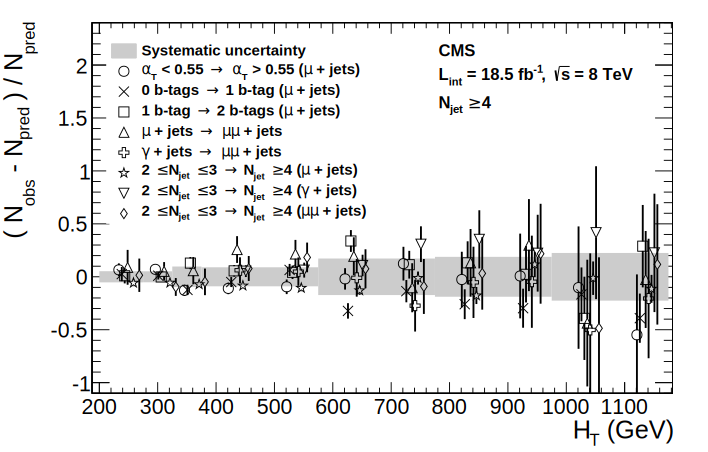
\includegraphics[width=0.505\textwidth]{figures/closure/summary_plot_njge4} 
%    } \\
%    \caption{ Sets of closure tests within and between different
%      control samples as a function of  $\scalht$ for (a) events with
%      up to three jets and (b) events with four or more jets.  \label{fig:closure} }
%  \end{center}
%\end{figure*}
%

The closure tests reveal no significant biases or dependencies on
\njet or \scalht for all individual tests. Systematic uncertainties in
the transfer factors are determined from the statistically-weighted
variance in the level of closure for collections of
tests.

Monte Carlo based templates are used to predict the background in the \mht distrbution. Control regions are used to evaluate the degree to which the Monte Carlo describes the variable in data and assign appropriate systematic uncertainties.

%Uncorrelated systematic uncertainties are determined for
%regions in \scalht and each jet multiplicity category, as defined in
%Table~\ref{tab:syst-values}.  An independent study to assess the
%effect of uncertainties in the simulation modelling of the efficiency
%and mistag rates for identifying jets originating from b-quarks and
%light-flavour partons on the transfer factors is also performed and
%found to be negligible, at the sub-percent level, with respect to the
%values quoted in Table~\ref{tab:syst-values}. The same (uncorrelated)
%value of systematic uncertainty is assumed for each \nb category.

%\begin{table}[!h]
%  \caption{Systematic uncertainties (\%) in the transfer factors,
%    according to \njet and \scalht region.}
%  \label{tab:syst-values}
%  \centering
%  \footnotesize
%  \begin{tabular}{ cccccccc }
%    \hline
%    \hline
%            & \multicolumn{7}{c}{\scalht region (GeV)}                                \\
%    \cline{2-8}
%    \njet   & 200--275 & 275--325 & 325--375 & 375--575 & 575--775 & 775-975 & $>975$ \\
%    \hline                                                                                                                                  
%    2--3    & 4        & 6        & 6        & 8        & 12       & 17      & 19     \\
%    $\geq$4 & 6        & 6        & 11       & 11       & 18       & 20      & 26     \\
%    \hline                                                                                                                                  
%    \hline
%  \end{tabular}
%\end{table}

%%__________________________________________________________________||

\section{Interpretation} 
\label{sec:interpretations}

\subsection{Specification for simplified models} 

The results of the search are used to constrain simplified
SUSY models~\cite{Alwall:2008ag, Alwall:2008va, sms}. Each
model assumes the pair production of gluinos or squarks and their
subsequent prompt decays to SM particles and the LSP ($\chiz_1$) with
a 100\% branching fraction (unless indicated otherwise). The gluino
decays contain intermediate on-shell SUSY particle states (such as the top
squark, $\PSQt$, or the chargino, $\chipm_1$) for a subset of the
models. All other SUSY particles are assumed to be too heavy ($m_{\sGlu} /
m_{\PSQ} = 10\TeV$) to be produced directly. Three-body decays of
gluinos are assumed to occur via off-shell squarks of light or heavy
flavour. Off-shell decays are processed by \PYTHIA in a single three-
or four-body step, without taking into account the width or
polarisation of the parent: this is true for the top squark four-body
decay ($\PSQt \ra \text{bf}\bar{\text{f}}'\chiz_1$), as well as the
three-body decay of the chargino ($\chipm_1 \ra
\text{f}\bar{\text{f}}'\chiz_1$), where f and f$'$ are fermions
produced in the decay of an intermediate off-shell W boson. 
%All SM particles with a finite lifetime, such as the W boson, are
%assumed to decay naturally.

\begin{table*}[!b]
  \topcaption{A summary of the simplified SUSY models used
    to interpret the results of this search. All on-shell SUSY particles
    in the decay are stated.} 
  \label{tab:simplified-models}
  \centering
  \footnotesize
  \begin{tabular}{ llll }
    \hline
Model class               %     & Fig.
                                & Production
                                & Decay
                                & Additional assumptions                                                         \\ [0.5ex]
\hline
\multicolumn{4}{l}{\it Gluino-mediated and direct production of light-flavour squarks}                           \\ [0.5ex]
\texttt{T1qqqq}        %        & \ref{fig:T1qqqq_feyn}                                                  
                                & $\text{pp}\ra\sGlu\sGlu$
                                & $\sGlu\ra\cPaq\cPq\chiz_1$
                                & --                                                                             \\ [0.5ex]
\texttt{T2qq\_8fold}   %        & \ref{fig:T2qq_feyn}                     
                                & $\text{pp}\ra\PSQ\PASQ$        
                                & $\PSQ\ra\cPq\chiz_1$
                                & $m_{\PSQ} = m_{\PSQ_\cmsSymbolFace{L}} = m_{\PSQ_\cmsSymbolFace{R}}$,
                       $\PSQ = \{ \PSQu, \PSQd, \PSQs, \PSQc \}$                                                 \\ [0.5ex]
\texttt{T2qq\_1fold}   %        & \ref{fig:T2qq_feyn}                                                  
                                & $\text{pp}\ra\PSQ\PASQ$         
                                & $\PSQ\ra\cPq\chiz_1$
                                & $m_{\PSQ (\PSQ \neq \PSQu_\cmsSymbolFace{L})} \gg m_{\PSQu_\cmsSymbolFace{L}}$ \\ [0.5ex]
\multicolumn{4}{l}{\it Gluino-mediated production of off-shell third-generation squarks}                         \\ [0.5ex]
\texttt{T1bbbb}        %        & \ref{fig:T1bbbb_feyn}                                                   
                                & $\text{pp}\ra\sGlu\sGlu$       
                                & $\sGlu\ra\cPaqb\cPqb\chiz_1$
                                & --                                                                             \\ [0.5ex]
\texttt{T1tttt}        %        & \ref{fig:T1tttt_feyn}
                                & $\text{pp}\ra\sGlu\sGlu$       
                                & $\sGlu\ra\cPaqt\PSQt^*\ra\cPaqt\cPqt\chiz_1$
                                & --                                                                             \\ [0.5ex]
\texttt{T1ttbb}        %        & \ref{fig:T1ttbb_feyn} 
                                & $\text{pp}\ra\sGlu\sGlu$      
                                & $\sGlu\ra\cPaqt\cPqb\chipm_1\ra\cPaqt\cPqb\PW^*\chiz_1$
                                & $m_{\chipm_1} - m_{\chiz_1} = 5\GeV$                                           \\ [0.5ex]
\multicolumn{4}{l}{\it Natural gluino-mediated production of on-shell top squarks}                               \\ [0.5ex]
\texttt{T5tttt\_DM175}        % & \ref{fig:T5tttt_feyn}
                                & $\text{pp}\ra\sGlu\sGlu$      
                                & $\sGlu\ra\cPaqt\PSQt\ra\cPaqt\cPqt\chiz_1$ 
                                & $m_{\,\PSQt} - m_{\chiz_1} = 175\GeV$                                          \\ [0.5ex]
\texttt{T5ttcc}        %        & \ref{fig:T5ttcc_feyn}            
                                & $\text{pp}\ra\sGlu\sGlu$       
                                & $\sGlu\ra\cPaqt\PSQt\ra\cPaqt\cPqc\chiz_1$ 
                                & $m_{\,\PSQt} - m_{\chiz_1} = 20\GeV$                                           \\ [0.5ex]
%\texttt{T5tttt\_degen} %       & \ref{fig:T5tttt_degen_feyn}
%                               & $\text{pp}\ra\sGlu\sGlu$      
%                               & $\sGlu\ra\cPaqt\PSQt\ra\cPaqt\cPqb\PW^*\chiz_1$
%                               & $m_{\,\PSQt} - m_{\chiz_1} = 20\GeV$                                           \\ [0.5ex]
\multicolumn{4}{l}{\it Direct production of on-shell third-generation squarks}                                   \\ [0.5ex]
\texttt{T2bb}          %        & \ref{fig:T2bb_feyn}
                                & $\text{pp}\ra\PSQb\PASQb$     
                                & $\PSQb\ra\cPqb\chiz_1$
                                & --                                                                             \\ [0.5ex]
\texttt{T2tb}          %        & \ref{fig:T2tb_feyn}
                                & $\text{pp}\ra\PSQt\PASQt$     
                                & $\PSQt\ra\cPqt\chiz_1 \;\text{or}\; \cPqb\chipm_1\ra\cPqb\PW^*\chiz_1$
                                & $50/50\%$, $m_{\chipm_1} - m_{\chiz_1} = 5\GeV$                                \\ [0.5ex]
\texttt{T2tt}          %        & \ref{fig:T2tt_feyn}
                                & $\text{pp}\ra\PSQt\PASQt$
                                & $\PSQt\ra\cPqt\chiz_1$
                                & --                                                                             \\ [0.5ex]
\texttt{T2cc}          %        & \ref{fig:T2cc_feyn}
                                & $\text{pp}\ra\PSQt\PASQt$      
                                & $\PSQt\ra\cPqc\chiz_1$
                                & $10 < m_{\,\PSQt} - m_{\chiz_1} < 80\GeV$                                      \\ [0.5ex]
\texttt{T2tt\_degen}   %        & \ref{fig:T2tt_degen_feyn}
                                & $\text{pp}\ra\PSQt\PASQt$      
                                & $\PSQt\ra\cPqb\PW^*\chiz_1$
                                & $10 < m_{\,\PSQt} - m_{\chiz_1} < 80\GeV$                                      \\ [0.5ex]
\texttt{T2tt\_mixed}   %        & \ref{fig:T2tt_mixed_feyn}
                                & $\text{pp}\ra\PSQt\PASQt$      
                                & $\PSQt\ra\cPqc\chiz_1 \;\text{or}\; \cPqb\PW^*\chiz_1$
                                & $50/50\%$, $10 < m_{\,\PSQt} - m_{\chiz_1} < 80\GeV$                           \\ [0.5ex]
    \hline
  \end{tabular}
\end{table*}

Fourteen unique production and decay modes are considered, which yield
a range of topologies and final states (with only the all-jet final
state considered in this search). Each class of simplified model is
identified by a label that indicates the topology and final state, and
scans in the gluino or squark ($m_{\sGlu} / m_{\PSQ}$) and LSP
($m_{\chiz_1}$) mass parameter space are performed.
%and the production and decay mode is indicated by the diagrams shown
%in Fig.~\ref{fig:simplified-models}. 
Table~\ref{tab:simplified-models} summarises the production and decay
modes, as well as any additional assumptions that define the
simplified models. The models can be categorised according to the
following descriptions: the gluino-mediated and direct production of
light-flavour squarks, the gluino-mediated production of off-shell
third-generation squarks, the ``natural'' gluino-mediated production
of on-shell top squarks, and the direct production of on-shell
third-generation squarks. In the case of direct pair production of
light-flavour squarks, two different assumptions on the theoretical 
production cross section are made. For the ``eightfold'' scenario
(\texttt{T2qq\_8fold}), the scalar partners to left- and right-handed
quarks of the u, d, s, and c flavours are assumed to be light and
degenerate in mass, with other squark states decoupled to a high
mass. For the ``onefold'' scenario (\texttt{T2qq\_1fold}), only a
single light squark is assumed to participate in the interaction and
all other squarks are decoupled to a high mass.

Under the signal+background hypothesis, and in the presence of a
nonzero signal contribution, a modified frequentist approach is used
to determine upper limits at the 95\% confidence level (CL) on the
cross section, $\sigma_\text{UL}$ (pb), to produce pairs of SUSY
particles as a function of the parent SUSY particle and the LSP
masses. The limits can be expressed in terms of the signal strength
parameter, $\mu$, which is determined relative to the theoretical
cross section that is calculated at NLO+NLL accuracy. An Asimov data
set~\cite{Cowan:2010js} is used to determined the expected upper limit
on the allowed cross section for a given model.  The potential
contributions from a new-physics signal to each of the signal and
control regions are considered, even though the only significant
contribution occurs in the signal region and not in the control
regions (\ie signal contamination). The approach is based on the
one-sided (so called LHC-style) profile likelihood ratio as the test
statistic~\cite{CMS-NOTE-2011-005} and the \cls criterion~\cite{junk,
  read}. Asymptotic formulae~\cite{Cowan:2010js} are utilised to
approximate the distributions of the test statistics under the SM
background-only and signal+background hypotheses.

%The test statistic is $q_\mu = -2 \ln (\mathcal{L}_\mu /
%\mathcal{L}_\text{max})$, where $\mathcal{L}_\text{max}$ is the
%maximum likelihood determined by allowing all parameters including a
%multiplier $\mu$ on the production cross section (``signal strength'')
%to vary, and $\mathcal{L}_\mu$ is the maximum likelihood for a fixed
%signal strength. To set limits, we use asymptotic results for the test
%statistic [71] and the \cls method described in Refs. [72, 73]. More
%details are provided in Refs. [15, 74].

\begin{table*}[!t]
  \topcaption{A summary of benchmark simplified models, the most sensitive
    \njet categories, and representative values for the corresponding
    experimental acceptance times efficiency
    ($\mathcal{A}\times\varepsilon$), the dominant systematic
    uncertainties, the theoretical production cross section
    ($\sigma_\text{theory}$), and the expected and observed upper limits
    on the production cross section, expressed in terms of the signal
    strength parameter ($\mu$).
  }
  \label{tab:signal-eff}
  \centering
  \footnotesize
  \begin{tabular}{ lllcrrrrrcc }
    \hline
    \multicolumn{2}{l}{Benchmark models} 
  & Most sensitive
  & $\mathcal{A}\times\varepsilon$
  & \multicolumn{4}{c}{Systematic uncertainties [\%]}
  & $\sigma_\text{theory}$
  & \multicolumn{2}{c}{$\mu$ (95\% CL)}                                                                           \\ [0.3ex]
    \cline{5-8}
    \multicolumn{2}{l}{$(m_{\text{SUSY}}, m_{\mathrm{LSP}})$ [GeV]} 
  & \njet categories
  & [\%]    
  & MC stat.
  & ISR 
  & JEC
  & $\text{SF}_\text{b-tag}$
  & \multicolumn{1}{c}{[fb]}
  & Exp.
  & Obs.                                                                                                          \\ [0.3ex] 
    \hline
    \multirow{2}{*}{\texttt{T1qqqq}} 
  & (1300, 100) & $\geq$5, 4, 3, 2         & \phantom{1}9.4 & 7-30  & $\sim$2 & 4-21  & 2-14 & 46.1 & 0.79 & 0.76 \\
  & (900, 700)  & $\geq$5, $\geq$5a, 4, 4a & \phantom{1}5.6 & 10-33 & 1-13    & 1-26  & 1-10 & 677  & 0.58 & 0.44 \\ [0.5ex]
%    \multirow{2}{*}{\texttt{T2qq\_8fold}}
% & (1050, 100) & $\geq$5, 3, 2, 4         & 13.4           & 7-33  & 2-5     & 3-16  & 1-11 & 44.0 & 0.72 & 0.50 \\
% & (650, 550)  & $\geq$5, 4, $\geq$5a, 4a & \phantom{1}2.6 & 10-28 & 3-9     & 2-28  & 1-6  & 1080 & 0.74 & 0.64 \\ [0.5ex]
%     \multirow{2}{*}{\texttt{T2qq\_1fold}}
% & (1050, 100) & $\geq$5, 3, 2, 4         & 17.9           & 7-33  & 2-5     & 3-16  & 1-11 & 44.0 & 0.72 & 0.50 \\
% & (650, 550)  & $\geq$5, 4, $\geq$5a, 4a & \phantom{1}2.6 & 10-28 & 3-9     & 2-28  & 1-6  & 1080 & 0.74 & 0.64 \\ [0.5ex]
  \multirow{2}{*}{\texttt{T2qq\_8fold}}
  & (1050, 100) & $\geq$5, 3, 4, 2         & 17.9           & 7-33  & 1-4     & 3-16  & 1-11 & 35.2 & 0.90 & 0.63 \\
  & (650, 550)  & $\geq$5, 4, $\geq$5a, 4a & \phantom{1}2.6 & 10-28 & 1-16     & 2-29  & 1-6  & 864  & 0.93 & 0.80 \\ [0.5ex]
  \multirow{2}{*}{\texttt{T2qq\_1fold}}
  & (600, 50)   & $\geq$5, 3, 2, 4         & 13.4           & 5-33  & 1-5     & 1-30  & 1-8  & 177  & 0.78 & 0.84 \\
  & (400, 250)  & $\geq$5, 4, $\geq$5a, 3  & \phantom{1}2.9 & 8-30  & 1-8     & 3-25  & 1-7  & 1849 & 0.73 & 0.71 \\ [0.5ex]
    \multirow{2}{*}{\texttt{T1bbbb}}
  & (1500, 100) & $\geq$5, 4, 3, 2         & 10.1           & 5-17  & 1-2     & 1-12  & 2-22 & 14.2 & 0.81 & 0.79 \\
  & (1000, 800) & $\geq$5, 4, $\geq$5a, 4a & \phantom{1}4.9 & 8-31  & 1-17    & 1-40  & 1-14 & 325  & 0.33 & 0.32 \\ [0.5ex]
    \multirow{2}{*}{\texttt{T1tttt}}
  & (1300, 100) & $\geq$5, $\geq$5a, 4, 3  & \phantom{1}2.4 & 7-16  & 1-2     & 2-7   & 2-12 & 46.1 & 1.00 & 1.89 \\
  & (800, 400)  & $\geq$5, $\geq$5a, 4, 4a & \phantom{1}0.6 & 7-27  & 1-2     & 3-45  & 1-8  & 1490 & 0.56 & 1.03 \\ [0.5ex]
    \multirow{2}{*}{\texttt{T1ttbb}}
  & (1300, 100) & $\geq$5, 4, 3, $\geq$5a  & \phantom{1}3.8 & 9-32  & 1-2     & 3-16  & 2-19 & 46.1 & 0.60 & 0.91 \\
  & (1000, 700) & $\geq$5, $\geq$5a, 4, 3  & \phantom{1}3.4 & 9-30  & 1-9     & 3-65  & 1-14 & 325  & 0.51 & 0.70 \\ [0.5ex]
    \multirow{2}{*}{\texttt{T5tttt\_DM175}}
  & (800, 100)  & $\geq$5, $\geq$5a, 3, 4  & \phantom{1}0.2 & 12-20 & 2-4     & 3-5   & 1-6  & 1490 & 0.69 & 1.19 \\
  & (700, 400)  & $\geq$5, $\geq$5a, 4, 4a & \phantom{1}0.2 & 20-29 & 2-10    & 8-10  & 1-2  & 3530 & 1.00 & 1.35 \\ [0.5ex]
% & (700, 400)  & $\geq$5, $\geq$5a, 4, 4a & \phantom{1}0.2 & 20-20 & 2-10    & 10-10 & 2-2  &      & 1.00 & 1.35 \\ [0.5ex]
% T5ttttDM175 (700,400)
%  Efficiency      0.2   0.3
%  isrSignalWeight 1.0   10.0
%  jecWeight       8.0   62.0
%  puWeight        1.0   22.0
%  bsfWeight       1.0   23.0
%  triggerWeight   6.0   19.0
%  mcStat          29.0  50.0
    \multirow{2}{*}{\texttt{T5ttcc}}  
  & (1200, 200) & $\geq$5, 4, 3, $\geq$5a  & \phantom{1}4.9 & 6-25  & 5-25    & 3-21  & 1-24 & 85.6 & 0.58 & 0.87 \\
  & (750, 600)  & $\geq$5, $\geq$5a, 4, 4a & \phantom{1}1.0 & 9-23  & 1-4     & 5-21  & 1-3  & 2270 & 0.89 & 0.72 \\ [0.5ex]
%    \multirow{2}{*}{\texttt{T5tttt\_degen}} 
% & (1100, 100) & $\geq$5, 4, 3, 4a        & \phantom{1}1.3 & 15-21 & 12-16   & 6-11  & 4-15 & 16.3 & 0.89 & 2.55 \\
% & (800, 600)  & $\geq$5, $\geq$5a, 4a, 4 & \phantom{1}1.9 & 5-32  & 1-8     & 1-34  & 1-7  & 1490 & 0.66 & 0.70 \\ [0.5ex]
    \multirow{2}{*}{\texttt{T2bb}}
  & (800, 50)   & 2, 3, 4, $\geq$5         & \phantom{1}1.5 & 5-31  & 2-6     & 1-21  & 1-23 & 28.3 & 0.96 & 1.06 \\
  & (375, 300)  & $\geq$5, 4, 3a, 3        & \phantom{1}0.1 & 8-33  & 1-10    & 3-25  & 1-7  & 2610 & 0.67 & 0.87 \\ [0.5ex]
    \multirow{2}{*}{\texttt{T2tb}}
  & (600, 50)   & $\geq$5, 4, 3, 2         & \phantom{1}6.1 & 3-28  & 1-3     & 1-22  & 1-17 & 175  & 0.70 & 1.35 \\
  & (350, 225)  & $\geq$5, 4, 3, 3a        & \phantom{1}1.0 & 9-33  & 1-4     & 2-41  & 1-8  & 3790 & 0.79 & 0.88 \\ [0.5ex]
    \multirow{2}{*}{\texttt{T2tt}}
  & (700, 50)   & $\geq$5, 4, 3, $\geq$5a  & \phantom{1}8.1 & 8-33  & 1-4     & 2-22  & 1-21 & 67.0 & 0.90 & 1.19 \\
  & (350, 100)  & $\geq$5, $\geq$5a, 4a, 4 & \phantom{1}1.4 & 7-31  & 1-1     & 1-28  & 1-7  & 3790 & 0.44 & 0.50 \\ [0.5ex]
    \multirow{1}{*}{\texttt{T2cc}}
  & (325, 305)  & $\geq$5, 4, 3, 2         & \phantom{1}0.8 & 3-32  & 1-27    & 1-27  & 1-12 & 5600 & 0.92 & 0.68 \\ [0.5ex]
    \multirow{1}{*}{\texttt{T2tt\_degen}}
  & (300, 290)  & 3, 4, $\geq$5, 2         & \phantom{1}0.9 & 2-27  & 1-27    & 1-25  & 1-12 & 8520 & 0.56 & 0.41 \\ [0.5ex]
    \multirow{1}{*}{\texttt{T2tt\_mixed}}
  & (300, 250)  & $\geq$5, 4, $\geq$5a, 4a & \phantom{1}0.4 & 3-33  & 1-27    & 1-33  & 1-13 & 8520 & 0.99 & 0.58 \\ [0.5ex]
    \hline
  \end{tabular}
\end{table*}

\subsection{Acceptances and uncertainties}

The experimental acceptance times efficiency
($\mathcal{A}\times\varepsilon$) and its uncertainty are evaluated
independently for each model class as a function of ($m_\text{SUSY},
m_\text{LSP}$). Table~\ref{tab:signal-eff} summarises
$\mathcal{A}\times\varepsilon$ for a number of benchmark models for
which the search yields an expected exclusion ($\mu \lesssim 1$). For
each topology, typically two different pairs of parent SUSY particle and
LSP masses ($m_\text{SUSY}, m_\text{LSP}$) are chosen that are
characterised by a large and a small (\ie ``compressed'') difference
in parent SUSY particle and LSP masses. The four most sensitive event
categories, defined in terms of \njet, are used to determine
$\sigma_\text{UL}$. The categories used per benchmark model are listed
in Table~\ref{tab:signal-eff}, along with
$\mathcal{A}\times\varepsilon$ determined for these four categories.

Contributions from several sources to the uncertainty in
$\mathcal{A}\times\varepsilon$ are considered. Each source of
uncertainty is included in the likelihood function via alternative
shapes to the nominal \HTmiss templates evaluated from simulated
signal events categorised according to \njet, \nb, and
\scalht. Correlations are taken into account where appropriate,
including those relevant to signal contamination in the control
regions. The morphing scheme that interpolates between the nominal and
alternative \HTmiss templates, described in Section~\ref{sec:result},
is also used for the simulated signal samples.

In addition to the uncertainty in the integrated luminosity of
2.7\%~\cite{CMS:2016eto}, the following sources of uncertainty are
dominant: the statistical uncertainty arising from the finite size of
simulated signal samples, the modelling of ISR, the jet energy
corrections (JEC) evaluated in simulation, and the modelling of scale
factors applied to simulated event samples that correct for
differences in the efficiency and misidentification probability of
b-quark jets ($\text{SF}_\text{b-tag}$). The magnitude of each
contribution depends on the model and the masses of the parent
SUSY particle and LSP.

The $\mathcal{A}\times\varepsilon$ for models with small mass
splittings (\eg $m_{\PSQ} - m_{\chiz_1} \lesssim m_{\text t}$) is due
largely to ISR, the modelling of which is evaluated by comparing the
simulated and measured \Pt spectra of the system recoiling against the
ISR jets in \ttbar events, using the technique described in
Ref.~\cite{single-lepton-stop}. The uncertainty can be as large as
$\sim$30\%, and is the dominant systematic uncertainty for systems
with a compressed mass spectrum. Uncertainties in the jet energy
scale, as large as $\sim$40\%, can also be dominant for models
characterised by high jet multiplicities in the final state. The
uncertainties in $\text{SF}_\text{b-tag}$ can be as large as
$\sim$25\%. Table~\ref{tab:signal-eff} summarises these dominant
contributions to the uncertainty in $\mathcal{A}\times\varepsilon$ for
a range of benchmark models. Characteristic values for each model are
expressed in terms of a range that is representative of the values
across all bins of the signal region. The upper bound for each range
may be subject to moderate statistical fluctuations.

Further uncertainties with subdominant contributions are considered on
a similar footing. The uncertainties in the efficiency of identifying
well-reconstructed, isolated leptons are considered, with a typical
magnitude of $\sim$5\% and treated as anticorrelated between the
signal and control regions. The uncertainty of 5\% in
$\sigma_\text{in}$ is propagated through to the reweighting procedure
to account for differences between the simulated and measured
pileup. Finally, uncertainties in the simulation modelling of the
efficiencies of the trigger strategy employed by the search are
typically $<$10\%. 

The choice of PDF set, or variations therein, predominantly affects
$\mathcal{A}\times\varepsilon$ through changes in the \Pt spectrum of
the system recoil, which is covered by the ISR uncertainty, hence no
additional uncertainty is adopted. Uncertainties in
$\mathcal{A}\times\varepsilon$ due to variations in the
renormalisation and factorisation scales are determined to be
relatively small. In both cases, contributions to the uncertainty in
the theoretical production cross section are considered.

\subsection{Cross section and mass exclusions}

%The upper limits on the signal production cross section are evaluated
%at a 95\% CL for each of the aforementioned benchmark models. The
%limits are expressed in terms of the signal strength parameter, $\mu$,
%which is determined relative to the theoretical cross section that is
%calculated at NLO+NLL accuracy. 

Limits for each of the aforementioned benchmark models are summarised
in Table~\ref{tab:signal-eff}, expressed in terms of $\mu$. All
benchmark models are expected to be excluded. The observed limits
fluctuate around the expected $\mu$ values, with some models
exhibiting a moderately weaker than expected limit.

\begin{figure*}[h!]
  \begin{center}
    \includegraphics[width=0.55\textwidth]{figures/limits/v3/mixSUMMARY.pdf}
    \includegraphics[width=0.55\textwidth]{figures/limits/v3/gluinoSUMMARY.pdf} 
    \caption{Observed and expected mass exclusions at 95\% CL
      (indicated, respectively, by solid and dashed contours) for
      various classes of simplified models. (Upper) Gluino-mediated or
      direct pair production of light-flavour squarks. The two
      scenarios involve, respectively, the decay
      $\sGlu\ra\cPaq\cPq\chiz_1$ (\texttt{T1qqqq}) and
      $\PSQ\ra\cPq\chiz_1$, and the latter involves two assumptions on
      the mass degeneracy of the squarks (\texttt{T2qq\_8fold} and
      \texttt{T2qq\_1fold}). (Lower) Three scenarios involving the
      gluino-mediated pair production of off-shell third-generation
      squarks: $\sGlu\ra\cPaqb\cPqb\chiz_1$ (\texttt{T1bbbb}),
      $\sGlu\ra\cPaqt\PSQt^*\ra\cPaqt\cPqt\chiz_1$ (\texttt{T1tttt}),
      and $\sGlu\ra\cPaqt\cPqb\chipm_1\ra\cPaqt\cPqb\PW^*\chiz_1$
      (\texttt{T1ttbb}).  }
    \label{fig:limits-sms-1} 
    \vspace{2.0cm} % hack to remove text from same page
  \end{center}
\end{figure*}

\begin{figure*}[h!]
  \begin{center}
    \includegraphics[width=0.53\textwidth]{figures/limits/v3/naturalWT1SUMMARY.pdf}
%    \includegraphics[width=0.6\textwidth]{figures/limits/v3/naturalSUMMARY.pdf}
    \includegraphics[width=0.53\textwidth]{figures/limits/v3/allThirdGenSUMMARY.pdf} 
    \caption{ Observed and expected mass exclusions at 95\% CL
      (indicated, respectively, by solid and dashed contours) for a
      number of simplified models. (Upper) Two scenarios involving the
      gluino-mediated pair production of on-shell top squarks:
      $\sGlu\ra\cPaqt\PSQt\ra\cPaqt\cPqt\chiz_1$ with $m_{\,\PSQt} -
      m_{\chiz_1} = 175\GeV$ (\texttt{T5tttt\_DM175}) and
      $\sGlu\ra\cPaqt\PSQt\ra\cPaqt\cPqc\chiz_1$ with $m_{\,\PSQt} -
      m_{\chiz_1} = 20\GeV$ (\texttt{T5ttcc}). Also shown, for
      comparison, is \texttt{T1tttt}. (Lower) Six scenarios involving
      the direct pair production of third-generation squarks. The
      first scenario involves the pair production of bottom squarks,
      $\PSQb\ra\cPqb\chiz_1$ (\texttt{T2bb}). Two scenarios involve
      the decay of top squark pairs as follows: $\PSQt\ra\cPqt\chiz_1$
      or $\PSQt\ra\cPqb\chipm_1\ra\cPqb\PW^*\chiz_1$ with
      $m_{\chipm_1} - m_{\chiz_1} = 5\GeV$ and branching fractions
      $50/50\%$ (\texttt{T2tb}), or $\PSQt\ra\cPqt\chiz_1$
      (\texttt{T2tt}). The final three scenarios consider top squark
      decays under the assumption $10 < m_{\,\PSQt} - m_{\chiz_1} <
      80\GeV$: $\PSQt\ra\cPqc\chiz_1$ (\texttt{T2cc}),
      $\PSQt\ra\cPqb\PW^*\chiz_1$ (\texttt{T2tt\_degen}), and
      $\PSQt\ra\cPqc\chiz_1$ or $\PSQt\ra\cPqb\PW^*\chiz_1$ with
      branching fractions $50/50\%$ (\texttt{T2tt\_mixed}). The grey
      shaded region denotes \texttt{T2tt} models that are not
      considered for interpretation. }
    \label{fig:limits-sms-2} 
  \end{center} 
\end{figure*}

Figures~\ref{fig:limits-sms-1} and~\ref{fig:limits-sms-2} summarise
the disfavoured regions of the mass parameter space for the fourteen
classes of simplified models. These regions are derived by comparing
the upper limits on the measured fiducial cross section, corrected for
the experimental $\mathcal{A}\times\varepsilon$, with the theoretical cross
sections calculated at NLO+NLL accuracy in
$\alpha_\text{s}$~\cite{susynlo}. The former cross section value is
determined as a function of $m_{\sGlu}$ or $m_{\PSQ}$ and
$m_{\chiz_1}$, while the latter has a dependence solely on $m_{\sGlu}$
or $m_{\PSQ}$.
%For each simplifed model, exclusion contours in the mass plane are
%shown when evaluated with the observed data counts in the signal
%region (solid contours) and the expected counts based on an asimov
%data set (dashed contours).
The exclusion of models is evaluated using observed data counts in the
signal region (solid contours) and also expected counts based on an
Asimov data set (dashed contours).

Figure~\ref{fig:limits-sms-1} (upper) shows the excluded mass parameter
space for models that assume the gluino-mediated or direct production
of light-flavour squarks. The excluded region extends to higher masses
for the gluino-mediated production of light-flavour squarks
(\texttt{T1qqqq}), with respect to direct pair production when
assuming an eightfold degeneracy in mass (\texttt{T2qq\_8fold}), due
to a combination of a higher gluino pair production cross section and
a final state characterised by higher jet multiplicities, which are
exploited to provide better signal-to-background separation. The
excluded mass region is significantly reduced when assuming only a
single light squark (\texttt{T2qq\_1fold}), with limits weakening due
to the lower production cross section, compounded by the reduced
signal-to-background ratios achieved in the core of distributions in
the discriminating variables.

Figure~\ref{fig:limits-sms-1} (lower) shows the exclusion contours
for models that assume the gluino-mediated pair production of
off-shell third-generation squarks. For the topologies \texttt{T1tttt}
and \texttt{T1bbbb}, each gluino is assumed to undergo a three-body
decay via, respectively, an off-shell top or bottom squark to a
quark-antiquark pair of the same flavour and the $\chiz_1$. In the
case of \texttt{T1ttbb}, each gluino is assumed to undergo a
three-body decay to an on-shell chargino, $\chipm_1$, a bottom quark,
and a top antiquark. The chargino mass is defined relative to the
neutralino mass via the expression $m_{\chipm_1} - m_{\chiz_1} =
5\GeV$. The chargino decays promptly to the $\chiz_1$ and an off-shell
W boson. The excluded mass regions differ significantly for these
topologies, primarily due to the different number of (on-shell) W
bosons in their final states, resulting in the highest $\mathcal{A}
\times \varepsilon$ for \texttt{T1bbbb} and lowest for
\texttt{T1tttt}. Further, $\mathcal{A} \times \varepsilon$ has a
strong dependence on jet multiplicity, which is highest for
\texttt{T1tttt}, due to the \bdphi variable. An additional feature for
\texttt{T1ttbb} is the weakening of the mass limit at low values of
$m_{\chiz_1}$, when $m_{\chipm_1} = m_{\chiz_1} + 5\GeV \lesssim
m_\text{t}$. In this scenario, the $\chipm_1$ (and hence $\chiz_1$) is
not highly Lorentz boosted relative to the top quark resulting from
the three-body decay of the gluino. Hence, two $\chiz_1$ SUSY particles do
not carry away significant \ptvecmiss, which is instead realised
through W boson decays to neutrinos and ``lost'' leptons or $\tau$
leptons that decay to neutrinos and hadrons. The observed mass limits
for these topologies are up to $\sim$2 standard deviations weaker than
the expected limits. These differences are due to upward fluctuations
in data for two contiguous bins that satisfy the requirements $\njet
\geq 5$, $\nb \geq 2$, and $\scalht > 800\GeV$. This region has the
highest sensitivity to models involving gluino production and decays
to third-generation quarks (via on- or off-shell squarks). The
observed counts are consistent with statistical fluctuations and the
events do not exhibit anomalous nonphysical behaviour. The events are
distributed in \HTmiss consistent with expectation, hence models
characterised by high values of \HTmiss, such as \texttt{T1bbbb} with
$m_{\sGlu} \gg m_{\chiz_1}$ or $m_{\sGlu} \approx m_{\chiz_1}$, are
less compatible with the data counts in this high-\njet, \nb, and
\scalht region.

Figure~\ref{fig:limits-sms-2} (upper) shows exclusion contours for
models that assume gluino pair production, with each gluino decaying
to a top quark and an on-shell top squark, the latter of which decays
to SM particles and the LSP, $\chiz_1$. As discussed earlier, these
models can be considered as representations of a ``natural'' solution
to the little hierarchy problem. Two different scenarios are
considered for the decay of the top squarks. The
\texttt{T5tttt\_DM175} models assume a two-body decay to a top quark
and the $\chiz_1$, with the top squark mass defined relative to the
$\chiz_1$ as $m_{\PSQt} - m_{\chiz_1} = m_\text{t}$. Models that
satisfy $m_{\chiz_1} < 50\GeV$ are not considered here, as the
$\chiz_0$ particles carry very little momentum.  The \texttt{T5ttcc}
models assume $m_{\PSQt} - m_{\chiz_1} = 20\GeV$ and two-body decays
to a charm quark and the $\chiz_1$.
%This decay is one of two modes open to the top squark under this
%near-mass-degenerate scenario.
%For comparison, the limit contours for \texttt{T1tttt}, which assumes
%an off-shell top squark that is decoupled to a high mass, are also
%shown in Fig.~\ref{fig:limits-sms-2} (upper). 
%The expected mass exclusion regions for \texttt{T1ttcc} and
%\texttt{T5tttt\_degen} are comparable to that of \texttt{T1tttt}, but
%do exhibit some different behaviour. % NEED DETAILS HERE

Finally, Fig.~\ref{fig:limits-sms-2} (lower) shows exclusion contours
for models that assume the direct production of pairs of
third-generation squarks. For the \texttt{T2bb} models, bottom squarks
are pair produced and each decays to a bottom quark and the
$\chiz_1$. The \texttt{T2tt} models assume top squarks are pair
produced and each is assumed to undergo a two- or three-body decay to,
respectively, a top quark and the $\chiz_1$ when $m_{\PSQt} -
m_{\chiz_1} > m_\text{t}$ is satisfied, or a b quark, an on-shell W
boson, and the $\chiz_1$ for the condition $m_{\PW} < m_{\PSQt} -
m_{\chiz_1} < m_\text{t}$. Models that satisfy $\abs{m_{\PSQt} -
  m_\text{t} - m_{\chiz_1}} < 25\GeV$ and $m_{\PSQt} + m_{\chiz_1} <
375\GeV$ are not considered here, as $\sigma_\text{UL}$ is a strong
function of $m_{\PSQt} - m_{\chiz_1}$ in this low-$m_{\PSQt}$ region,
due to the high levels of signal contamination found in the \mj
control region for models that resemble the \ttbar background in terms
of their topological and kinematic properties. The \texttt{T2tb}
models also assume the pair production of top squarks, with each
undergoing a two-body decay to either a top quark and the $\chiz_1$,
or a bottom quark and the $\chipm_1$, with equal branching fractions
of 50\%. As for the \texttt{T1ttbb} models, the chargino mass is
defined relative to the neutralino mass via the expression
$m_{\chipm_1} - m_{\chiz_1} = 5\GeV$, and the chargino decays promptly
to the $\chiz_1$ and an off-shell W boson. The excluded mass regions
differ significantly for the \texttt{T2bb}, \texttt{T2tb}, and
\texttt{T2tt} topologies, in an analogous way to the \texttt{T1bbbb},
\texttt{T1ttbb}, and \texttt{T1tttt} models described above. The
difference in the mass exclusions is due primarily to the different
number of (on-shell) W bosons in the final states, which affects
$\mathcal{A} \times \varepsilon$ through the presence of leptons from
the decay of the W boson. An additional feature for \texttt{T2tb} is
the weakening of the mass limit at low values of $m_{\chiz_1}$, when
$m_{\chipm_1} = m_{\chiz_1} + 5\GeV \lesssim m_\text{t}$. Moderately
weaker than expected mass limits are observed for all models involving
two-body decays, which is traced to mild upward fluctuations in data
for events satisfying $\njet = 2$, $\nb = 2$, and $350 < \scalht <
500\GeV$.

Figure~\ref{fig:limits-sms-2} (lower) also shows exclusion contours
for models that assume the pair production of top squarks but a
near-mass-degenerate system that satisfies $10\GeV < m_{\PSQt} -
m_{\chiz_1} < m_\PW$. Two decays of the top squark are
considered. 
%Analogous to the \texttt{T5ttcc} and \texttt{T5tttt\_degen} models
%(but without the gluino), 
The \texttt{T2cc} and \texttt{T2tt\_degen} models assume two- and
four-body decays of the top squark to, respectively, a charm quark and
the $\chiz_1$, or to $\text{bf}\bar{\text{f}}'\chiz_1$, where
$\text{f}$ and $\bar{\text{f}}'$ are fermions produced in the decay of
an intermediate off-shell W boson. A third class of models,
\texttt{T2tt\_mixed}, assumes both these decay modes with an equal
branching fraction of 50\%. For \texttt{T2cc}, the excluded mass
region is relatively stable as a function of the mass splitting $\dm =
m_{\PSQt} - m_{\chiz_1}$, with $\PSQt$ masses excluded up to
400\GeV. For \texttt{T2tt\_degen}, the excluded mass region is
strongly dependent on \dm, weakening considerably for increasing
values of \dm due to the increased momentum phase space available to
leptons produced in the four-body decay. The \texttt{T2tt\_mixed}
models exhibit an intermediate behaviour. Mass limits for all three
model classes converge for the smallest mass splitting considered,
$\dm = 10\GeV$, when the SM particles from the \PSQt decay are
extremely soft and outside the experimental acceptance. An
approximately contiguous mass exclusion limit is observed across the
transition from the \texttt{T2tt\_degen} four-body to the
\texttt{T2tt} three-body decay of the $\PSQt$, as the top quark moves
on-shell. The excluded mass region weakens further as $\dm \ra
m_\text{t}$.

Table~\ref{tab:simplified-models-limits} summarises the strongest
expected and observed excluded $m_{\sGlu}$ or $m_{\PSQ}$ and
$m_{\chiz_1}$ masses for each class of simplified model.

\begin{table}[!t]
  \topcaption{Summary of the mass limits obtained for the fourteen 
    classes of simplified models. The limits indicate the strongest
    observed and expected (in parentheses) mass exclusions in $\sGlu$,
    $\PSQ$, $\PSQb$, $\PSQt$, and $\chiz_1$. The quoted values have
    uncertainties of $\pm$25 and $\pm$10\GeV for models involving
    the pair production of, respectively, gluinos and squarks.
  }
  \label{tab:simplified-models-limits}
  \centering
  \footnotesize
  \begin{tabular}{ lccc }
    \hline
    Model class & Parent    & \multicolumn{2}{c}{Best mass limit [GeV]}  \\
    \cline{3-4}
                & SUSY particle & $\sGlu / \PSQ / \PSQb / \PSQt$ & $\chiz_1$\T \\ [0.5ex]
    \hline
%    \multicolumn{4}{l}{\it Gluinos and light-flavour squarks}                         \\ 
%    \multicolumn{4}{l}{\it Gluinos and off-shell stops and sbottoms}                  \\ 
%    \multicolumn{4}{l}{\it Gluinos and on-shell stops}                                \\ 
%    \multicolumn{4}{l}{\it Direct top squark production}                              \\ 
    \texttt{T1qqqq}        & $\sGlu$   & 1375 \ph(1350)                 & 875 \ph(850) \\ 
    \texttt{T2qq\_8fold}   & $\PSQ$    & 1150 \ph(1075)                 & 600 \ph(550) \\ 
    \texttt{T2qq\_1fold}   & $\PSQ$    & \ph575 \ph\ph(650)             & 275 \ph(275) \\ 
    \texttt{T1bbbb}        & $\sGlu$   & 1575 \ph(1575)                 & 975 (1025)   \\ 
    \texttt{T1tttt}        & $\sGlu$   & 1125 \ph(1325)                 & 475 \ph(600) \\ 
    \texttt{T1ttbb}        & $\sGlu$   & 1375 \ph(1450)                 & 750 \ph(850) \\ 
    \texttt{T5tttt\_DM175}        & $\sGlu$   & \ph800 \ph(1000)               & 300 \ph(450) \\ 
    \texttt{T5ttcc}        & $\sGlu$   & 1350 \ph(1350)                 & 700 \ph(800) \\ 
%    \texttt{T5tttt\_degen} & $\sGlu$   & 1150 \ph(1275)                 & 650 \ph(725) \\ 
    \texttt{T2bb}          & $\PSQb$   & \ph800 \ph\ph(800)             & 360 \ph(400) \\ 
    \texttt{T2tb}          & $\PSQt$   & \ph610 \ph\ph(690)             & 240 \ph(300) \\ 
    \texttt{T2tt} (3-body) & $\PSQt$   & \ph670 \ph\ph(720)             & 210 \ph(240) \\
    \texttt{T2tt} (2-body) & $\PSQt$   & \ph280 \ph\ph(280)             & 200 \ph(200) \\ 
    \texttt{T2cc}          & $\PSQt$   & \ph400 \ph\ph(350)             & 310 \ph(340) \\ 
    \texttt{T2tt\_degen}   & $\PSQt$   & \ph370 \ph\ph(360)             & 360 \ph(350) \\ 
    \texttt{T2tt\_mixed}   & $\PSQt$   & \ph360 \ph\ph(350)             & 350 \ph(340) \\ [0.5ex]
    \hline
  \end{tabular}
\end{table}

















%%%%%%%%%%%%%%%%%%%%%%%%%%%%%%%%%%%%%%%%%%%%%%%%%%%%%%%%%%%%%%%%%%%%%%%%%%%%%%%%
%%%%%%%%%%%%%%%%%%%%%%%%%%%%%%%%%%%%%%%%%%%%%%%%%%%%%%%%%%%%%%%%%%%%%%%%%%%%%%%%
%%%%%%%%%%%%%%%%%%%%%%%%%%%%%%%%%%%%%%%%%%%%%%%%%%%%%%%%%%%%%%%%%%%%%%%%%%%%%%%%
%%%%%%%%%%%%%%%%%%%%%%%%%%%%%%%%%%%%%%%%%%%%%%%%%%%%%%%%%%%%%%%%%%%%%%%%%%%%%%%%

%\clearpage
%\begin{figure*}[tb]
%  \begin{center}
%    \subfigure[\texttt{T1qqqq}]{
%      \includegraphics[height=0.15\textwidth]{figures/diagrams/CMS_logo}
%      \label{fig:T1qqqq_feyn}
%    } ~~
%    \subfigure[\texttt{T2qq}]{
%      \includegraphics[height=0.15\textwidth]{figures/diagrams/T2qq_feyn}
%      \label{fig:T2qq_feyn}
%    } ~~
%    \subfigure[\texttt{T1bbbb}]{
%      \includegraphics[height=0.15\textwidth]{figures/diagrams/CMS_logo}
%      \label{fig:T1bbbb_feyn}
%    } ~~
%    \subfigure[\texttt{T1tttt}]{
%      \includegraphics[height=0.15\textwidth]{figures/diagrams/T1tttt_feyn}
%      \label{fig:T1tttt_feyn}
%    } ~~
%    \subfigure[\texttt{T1ttbb}]{
%      \includegraphics[height=0.15\textwidth]{figures/diagrams/T5ttbb_feyn}
%      \label{fig:T1ttbb_feyn}
%    } \\
%    \subfigure[\texttt{T5tttt\_DM175}]{
%      \includegraphics[height=0.15\textwidth]{figures/diagrams/T5tttt_feyn}
%      \label{fig:T5tttt_feyn}
%    } ~~
%    \subfigure[\texttt{T5ttcc}]{
%      \includegraphics[height=0.15\textwidth]{figures/diagrams/T5ttcc_feyn}
%      \label{fig:T5ttcc_feyn}
%    } ~~
%    \subfigure[\texttt{T5tttt\_degen}]{
%      \includegraphics[height=0.15\textwidth]{figures/diagrams/T5tttt_degen_feyn}
%      \label{fig:T5tttt_degen_feyn}
%    } ~~
%    \subfigure[\texttt{T2bb}]{
%      \includegraphics[height=0.15\textwidth]{figures/diagrams/T2bb_feyn}
%      \label{fig:T2bb_feyn}
%    } ~~
%    \subfigure[\texttt{T2tb}]{
%      \includegraphics[height=0.15\textwidth]{figures/diagrams/CMS_logo}
%      \label{fig:T2tb_feyn}
%    } \\
%    \subfigure[\texttt{T2tt}]{
%      \includegraphics[height=0.15\textwidth]{figures/diagrams/T2tt_feyn}
%      \label{fig:T2tt_feyn}
%    } ~~
%    \subfigure[\texttt{T2cc}]{
%      \includegraphics[height=0.15\textwidth]{figures/diagrams/CMS_logo}
%      \label{fig:T2cc_feyn}
%    } ~~
%    \subfigure[\texttt{T2tt\_degen}]{
%      \includegraphics[height=0.15\textwidth]{figures/diagrams/CMS_logo}
%      \label{fig:T2tt_degen_feyn}
%    } ~~
%    \subfigure[\texttt{T2tt\_mixed}]{
%      \includegraphics[height=0.15\textwidth]{figures/diagrams/CMS_logo}
%      \label{fig:T2tt_mixed_feyn}
%    } ~~
%    \caption{ Simplified model diagrams that represent unique
%      production and decay modes of SUSY 
%      particles. Three-body decays of gluinos are assumed to proceed
%      through off-shell squarks. Additional assumptions concerning the
%      mass relations and branching ratios are specified in
%      Table~\ref{tab:simplified-models}. The diagrams labelled
%      \texttt{T1qqqq} and \texttt{T2qq} depict, respectively, the
%      gluino-mediated and direct production of light-flavour
%      squarks. The diagrams labelled \texttt{T1bbbb}, \texttt{T1tttt},
%      and \texttt{T1ttbb} depict models involving the gluino-mediated
%      production of off-shell third-generation squarks. The diagrams
%      labelled \texttt{T5tttt\_DM175}, \texttt{T5ttcc}, and
%      \texttt{T5tttt\_degen} depict ``natural'' models comprising
%      gluino-mediated production of on-shell top squarks. Finally, the
%      remaining six diagrams depict the direct production of on-shell
%      third-generation squarks, decaying via a range of channels.  }
%    \label{fig:simplified-models}
%  \end{center}
%\end{figure*}




%& PU & Trigger & XS [pb] & XS [fb] (3sf)
%& 1-5  & 1-3  & 0.0460525 & 46.1             
%& 1-9  & 5-13 & 0.677478  & 677\phantom{.0}  
%                                             
%& 1-10 & 1-6  & 0.0439731 & 44.0             
%& 1-15 & 3-12 & 1.08047   & 1080\phantom{.0} 
%                                             
%& 1-4  & 1-3  & 0.0141903 & 14.2             
%& 1-20 & 1-15 & 0.325388  & 325\phantom{.0}  
%                                             
%& 1-4  & 1-3  & 0.0460525 & 46.1             
%& 1-13 & 1-10 & 1.4891    & 1490\phantom{.0} 
%                                             
%& 1-18 & 1-4  & 0.0460525 & 46.1             
%& 1-12 & 1-14 & 0.325388  & 325\phantom{.0}  
%                                             
%& 2-6  & 3-6  & 1.4891    & 1490\phantom{.0} 
%& 4-4  & 3-10 & 3.5251    & 3530\phantom{.0} 
%                                             
%& 1-9  & 2-6  & 0.0856418 & 85.6             
%& 1-8  & 4-7  & 2.26585   & 2270\phantom{.0} 
%                                             
%& 3-5  & 3-4  & 0.163491  & 16.3             
%& 1-20 & 1-11 & 1.4891    & 1490\phantom{.0} 
%                                             
%& 1-16 & 2-12 & 0.0283338 & 28.3             
%& 1-11 & 3-3  & 2.61162   & 2610\phantom{.0} 
%                                             
%& 1-8  & 1-12 & 0.174599  & 175\phantom{.0}  
%& 1-12 & 5-7  & 3.78661   & 3790\phantom{.0} 
%                                             
%& 1-13 & 2-11 & 0.0670476 & 67.0             
%& 1-10 & 5-9  & 3.78661   & 3790\phantom{.0} 
%                                             
%& 1-26 & 5-16 & 5.60471   & 5600\phantom{.0} 
%                                             
%& 1-11 & 2-18 & 8.51615   & 8520\phantom{.0} 
%                                             
%& 1-22 & 2-16 & 8.51615   & 8520\phantom{.0} 

%\clearpage
%\begin{figure*}[thp!]
%  \begin{center}
%    \includegraphics[width=0.49\textwidth]{figures/limits/v3/mixSUMMARY.pdf}
%    \includegraphics[width=0.49\textwidth]{figures/limits/v3/gluinoSUMMARY.pdf} \\
%    \includegraphics[width=0.49\textwidth]{figures/limits/v3/naturalSUMMARY.pdf}
%    \includegraphics[width=0.49\textwidth]{figures/limits/v3/allThirdGenSUMMARY.pdf} \\
%    \caption{Observed upper limit in cross section at 95\% CL
%      (indicated by the colour scale) for simplified models that
%      assume the pair production of gluinos, as a function of the
%      gluino and $\chiz_{1}$ masses for gluino three-body decays to
%      $b\bar{b}\chiz_{1}$ (top left), $q\bar{q}\chiz_{1}$ (top right) and $t\bar{t}\chiz_{1}$ (bottom center). 
%      The black solid thick (thin) line indicates the observed mass
%      exclusion region assuming the nominal (${\pm}1 \sigma$ theoretical
%      uncertainty) production cross section. The red dashed thick
%      (thin) line indicates the median (${\pm}1 \sigma$ experimental
%      uncertainty) expected exclusion.
%    }
%    \label{fig:limits-sms} 
%  \end{center}
%\end{figure*}



\section{Summary}
\label{sec:summary}

An inclusive search for new-physics phenomena is reported, based on
data from pp collisions at $\sqrt{s} = 13\TeV$. The data are recorded
with the CMS detector and correspond to an integrated luminosity of
$2.3 \pm 0.1 \fbinv$. The final states analysed contain one or more
jets with large transverse momenta (\Pt) and a significant imbalance
in transverse momentum, as expected from the production of massive
coloured sparticles, each decaying to SM particles and the lightest
stable, weakly-interacting supersymmetric particle.

Signal candidate events are categorised according to the number of
reconstructed jets, and the number of jets identified as originating
from b quarks, and the scalar (\scalht) and vector (\HTmiss) sums of
the transverse momenta of jets.  The search employs the use of several
kinematic variables, including \alphat and \bdphi, to suppress the
background from QCD multijet production to the percent level with
respect to other non-multijet SM backgrounds, which are dominated by
vector boson and top-antitop production. The \alphat variable is also
employed in the trigger logic that is used to record the candidate
signal events, which allows the use of low thresholds for the momentum
sums, $\scalht > 200\GeV$ and $\HTmiss \gtrsim 130\GeV$. These low
thresholds, in addition to the inclusion of final states containing a
single jet, maximise the experimental acceptance to new-physics
processes, such as low-mass squark signatures, nearly mass-degenerate
SUSY models, and other new-physics phenomena, such as DM models that
postulate the direct production of stable, weakly interacting, massive
particles in pp collisions.

The sums of the standard model backgrounds are estimated from a
simultaneous binned likelihood fit to the observed yields for samples
of events categorised according to \njet, \nb, \scalht, and \HTmiss in
the signal region and in \mj, \mmj, and \gj control regions. The
observed yields in the signal are found to be in agreement with the
expected contributions from standard model processes.  The search
result is interpreted in the mass parameter space of fourteen 
simplified supersymmetric models that assume the pair production of
gluinos or squarks and a range of decay modes. The models cover
scenarios that involve the gluino-mediated or direct production or
light- or heavy-flavour squarks, spectra with intermediate sparticle
states and branching ratios, ``natural'' spectra with gluinos and
on-shell top squarks, and nearly mass-degenerate spectra.

The increase in the centre-of-mass energy of the LHC, from $\sqrt{s} =
8$ to 13\TeV, provides a significant gain in sensitivity to heavy
particle states such as gluinos. In the case of pair production of
gluinos that each decays, via an off-shell b squark, to the b quark
and the LSP, models with masses up to $\sim$1.6\TeV and $\sim$1.0\TeV
are excluded for, respectively, the gluino and LSP, which is an
improvement of, respectively, $\sim$250 and $\sim$300\GeV with respect
to Run~1. In the case of direct pair production, models with masses up
to $\sim$800\GeV and $\sim$350\GeV are excluded for, respectively, the
b squark and LSP. These mass limits are sensitive to the assumptions
on the squark flavour and the presence of intermediate states, such as
charginos.

Finally, a comprehensive study of nearly mass-degenerate models
involving top squark pair production is performed. The two decay modes
open to the top squark are considered: the loop-induced two-body decay
to the neutralino and one c quark, and the four-body decay to the
neutralino, one b quark, and an off-shell W boson. A third scenario is
considered, when the two modes are simultaneously open each with a
branching ratio of 50\%. Masses of the top squark and LSP up to,
respectively, 400\GeV and 360\GeV are excluded, depending on the decay
modes considered.

In summary, the analysis provides sensitivity across a large region of
the ``natural'' supersymmetric parameter space, as characterised by
interpretations with several simplified models. In particular, these
studies improve on existing limits for nearly mass-degenerate models
involving the production of pairs of top squarks.


%%__________________________________________________________________||
% \nocite{*}
\bibliography{auto_generated}

%%__________________________________________________________________||
